% Báo cáo AS3179: khung theo template (trang bìa, đầu/chân trang, mục lục) và bố cục trong docs/report_outline.md.
% Biên dịch: pdfLaTeX với -shell-escape (cần cho gói minted): python scripts/04_build_report.py, hoặc Overleaf (compiler pdfLaTeX).
% Chương 1, 2, 3, 6, 7, tài liệu tham khảo, phụ lục: chapters/*.tex. Chương 4, 5 có hình/bảng chèn tự động từ reports/.
\documentclass[11pt]{article}
\usepackage[includeheadfoot,textheight=21cm,textwidth=17cm,headheight=10mm]{geometry}
\usepackage[vietnamese]{babel}
\usepackage{amsmath,amssymb}
\usepackage{xcolor,fancyhdr,indentfirst,array,graphicx,setspace,titlesec,tikz,float,booktabs,longtable,adjustbox,caption,enumitem,needspace,placeins,xurl}
\usepackage{minted}
\usepackage[hidelinks]{hyperref}

% --- đường dẫn hình/bảng (script 06 đổi ../figures, ../tables thành figures, tables cho Overleaf) ---
\newcommand{\figdir}{../figures}
\newcommand{\tabdir}{../tables}
\graphicspath{{assets/}}

% --- ký hiệu và macro dùng chung ---
\newcommand{\TODO}[1]{{\color{red}\textbf{[TODO(nhóm): #1]}}}
\newcommand{\figx}[2]{\begin{figure}[H]\centering\includegraphics[width=\linewidth]{\figdir/#1.png}\caption{#2}\label{fig:#1}\end{figure}}
% cấp 4: a), b), c)... (tự đánh chữ, đặt lại sau mỗi mục cấp 3)
\newcounter{noidung}[subsubsection]
\renewcommand{\thenoidung}{\alph{noidung}}
\newcommand{\noidung}[1]{\refstepcounter{noidung}\Needspace{8\baselineskip}\par\medskip\noindent\textbf{\thenoidung) #1}\par\smallskip}
% sáu thành phần của mỗi nội dung kiểm chứng và nhãn cấp 5: (i), (ii), (iii)
\newcommand{\tp}[1]{\par\smallskip\noindent\textbf{\textit{#1.}}\ }
\newcommand{\bodl}[1]{\par\noindent\textit{#1}\ }

% --- định dạng các cấp tiêu đề ---
\titleformat{\section}{\normalfont\Large\bfseries}{CHƯƠNG \thesection.}{0.6em}{}
\titleformat{\subsection}{\normalfont\large\bfseries}{\thesubsection}{0.6em}{}
\titleformat{\subsubsection}{\normalfont\normalsize\bfseries\itshape}{\thesubsubsection}{0.6em}{}
\titlespacing*{\section}{0pt}{0pt}{14pt}
\titlespacing*{\subsection}{0pt}{14pt}{6pt}
\titlespacing*{\subsubsection}{0pt}{10pt}{4pt}
\setcounter{secnumdepth}{3}
\setcounter{tocdepth}{3}
\counterwithin{figure}{section}
\counterwithin{table}{section}
\captionsetup{font=small,labelfont=bf}
\setstretch{1.15}
\setlength{\parindent}{1cm}
\renewcommand*{\contentsname}{\LARGE\textbf{Mục lục}}
\setminted{fontsize=\footnotesize,breaklines,frame=single}

\begin{document}

% ================= TRANG BÌA =================
\AddToHookNext{shipout/background}{
	\begin{tikzpicture}[remember picture,overlay]
		\node at (current page.center) {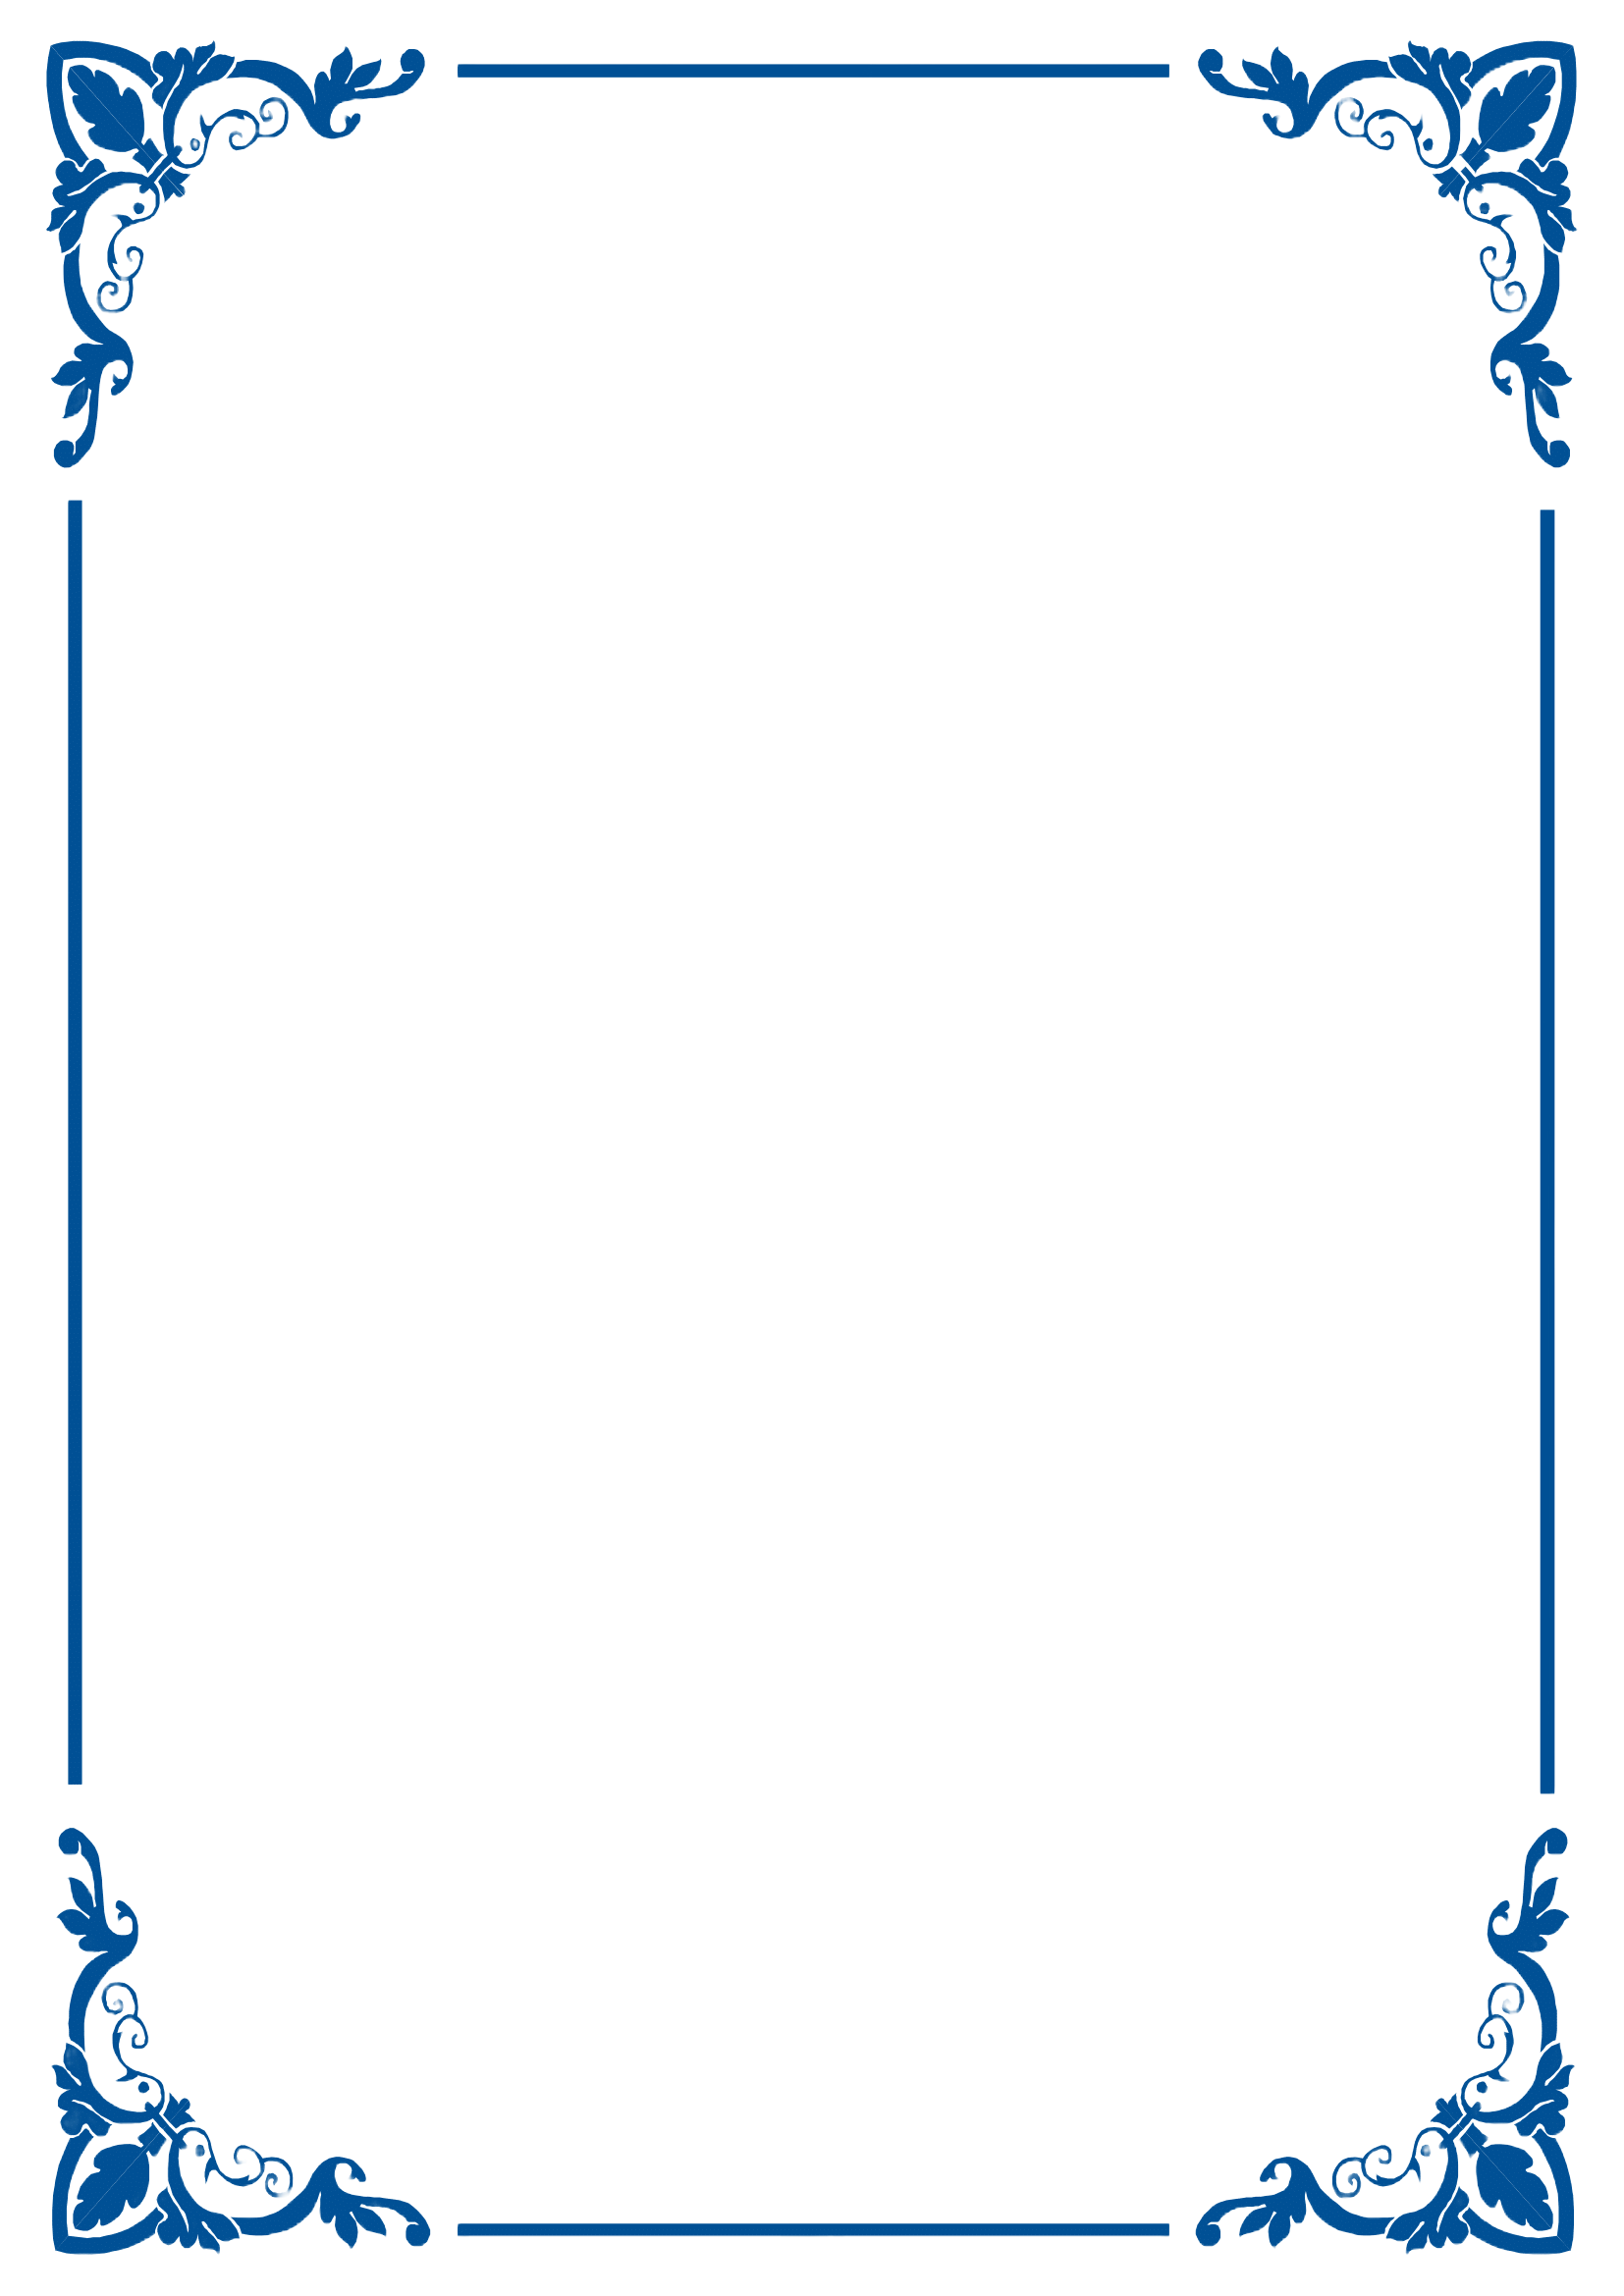
\includegraphics[width=19.4cm]{background.png}};
	\end{tikzpicture}
}
\thispagestyle{empty}
\begin{center}
	\textbf{\large ĐẠI HỌC QUỐC GIA THÀNH PHỐ HỒ CHÍ MINH\\
		TRƯỜNG ĐẠI HỌC BÁCH KHOA \\ KHOA KHOA HỌC ỨNG DỤNG \\\textunderscore\textunderscore\textunderscore\textunderscore\textunderscore\textunderscore\textunderscore\textunderscore\textunderscore\textunderscore\textunderscore\textunderscore\textunderscore}
\end{center}
\begin{figure}[h]
	\centering
	
\includegraphics[width=0.4\linewidth]{01_logobachkhoasang}
\end{figure}
\begin{center}
	\textbf{\Large MÔ HÌNH THỐNG KÊ (AS3179) \\}
	\LARGE
	\begin{center}
		\noindent\rule{450pt}{0.8pt}
		\vspace{0.5em}
		\begin{flushleft}
			\hspace{60pt}\textbf{\large Bài tập lớn:}
		\end{flushleft}
		{\LARGE\textbf{KIỂM CHỨNG THỰC NGHIỆM\\CÁC MÔ HÌNH ARMA VÀ ARIMA\\TRÊN DỮ LIỆU CHUỖI THỜI GIAN}}\\
		\noindent\rule{450pt}{0.8pt}
	\end{center}
	\textbf{\large HỌC KỲ \TODO{mã học kỳ} \\}
	\textbf{\large Giảng viên: \TODO{họ tên giảng viên}\\}
	\textbf{\large Chuyên đề: Mô hình chuỗi thời gian \TODO{giữ hay bỏ ``(cặp bài giảng 11--12)''}\\}
	\large
	\begin{flushleft}
		\hspace{1.5cm}\textbf{\large Danh sách sinh viên thực hiện: }
	\end{flushleft}
	\begin{center}
		\large
		\begin{tabular}{|c|c|c|c|c|}
			\hline
			\textbf{STT} & \textbf{\hspace{1cm}Họ\hspace{1cm}} & \textbf{Tên} & \hspace{0.3cm}\textbf{MSSV}\hspace{0.3cm} & \textbf{\hspace{1.5cm}Ghi chú\hspace{1.5cm}} \\
			\hline
			1 & \TODO{họ} & \TODO{tên} & \TODO{MSSV} & \\
			\hline
			2 & \TODO{họ} & \TODO{tên} & \TODO{MSSV} & \\
			\hline
			3 & \TODO{họ} & \TODO{tên} & \TODO{MSSV} & \\
			\hline
		\end{tabular}
	\end{center}
	\textbf{\textit{Thành phố Hồ Chí Minh, tháng 11 năm 2026.}}
\end{center}
\newpage

% ================= ĐẦU/CHÂN TRANG VÀ MỤC LỤC =================
\pagestyle{fancy}
\renewcommand{\footrulewidth}{1pt}
\fancyhead{}
\lhead{
\includegraphics[width=8cm]{bk_name_en}}
\rhead{\textbf{\large {\color{blue}Mô hình thống kê (AS3179)}\\ \small{Kiểm chứng thực nghiệm các mô hình ARMA và ARIMA}}}
\fancyfoot{}
\cfoot{Trang \thepage}
\setcounter{page}{1}

\tableofcontents
\newpage

% ================= NỘI DUNG =================
% CHƯƠNG 1. GIỚI THIỆU
\clearpage
\section[Giới thiệu]{GIỚI THIỆU}

Chuỗi thời gian xuất hiện ở khắp nơi: mực nước của một hồ lớn, lưu lượng của một dòng sông, số hành khách hàng không hay chỉ số chứng khoán.

\subsection{Bối cảnh}
Chuỗi thời gian là một dãy quan sát ghi theo thứ tự thời gian. Khác với dữ liệu thông thường, các quan sát liền nhau thường không độc lập: mực nước năm nay phụ thuộc mực nước năm trước, giá hôm nay liên quan đến giá hôm qua. Sự phụ thuộc này vừa là điều cần mô tả, vừa khiến các phương pháp dành cho dữ liệu độc lập không dùng được nguyên vẹn.

ARMA và ARIMA là công cụ nền tảng để mô tả sự phụ thuộc ấy và để dự báo. Lý thuyết của chúng dựa trên những giả thiết gọn, như chuỗi dừng, nhiễu có tính chất cho trước và mô hình đúng bậc, trong khi dữ liệu thực hiếm khi thỏa mãn hoàn hảo vì có thể trôi, đổi mức, có mùa vụ hoặc có biến động thay đổi theo thời gian. Câu hỏi tự nhiên là lý thuyết còn đúng đến đâu trên dữ liệu thực, và khi lệch thì lệch vì lý do gì. Báo cáo này đi tìm lời đáp cho câu hỏi đó.

\subsection{Mục tiêu}
Mục tiêu chung là kiểm chứng bằng Python các kết quả lý thuyết về chuỗi dừng, ARMA, chuỗi không dừng, ARIMA và dự báo trên sáu bộ dữ liệu thực, kết hợp mô phỏng khi cần, rồi đánh giá mức độ phù hợp giữa lý thuyết và thực nghiệm. Cụ thể, báo cáo trả lời ba câu hỏi sau:
\begin{enumerate}[label=\textbf{CH\arabic*:}]
	\item Các kết quả lý thuyết về cấu trúc phụ thuộc và mô hình ARMA có được thỏa mãn trên dữ liệu thực hay không?
	\item Các kết quả lý thuyết về chuỗi không dừng, mô hình ARIMA và dự báo có được thỏa mãn trên dữ liệu thực hay không?
	\item Mức độ phù hợp phụ thuộc thế nào vào đặc điểm của từng bộ dữ liệu, và giả thiết nào bị vi phạm?
\end{enumerate}

\subsection{Phạm vi}
Báo cáo dùng sáu bộ dữ liệu của R, được ký hiệu theo Danh mục ký hiệu và chữ viết tắt ở đầu báo cáo, và chỉ gọi bằng các ký hiệu ấy ở những phần sau. Hai ký hiệu DR và DP cùng chỉ số DAX nhưng ở hai dạng khác nhau, vì suất sinh lợi là dạng dừng còn log giá là dạng không dừng của cùng một chuỗi.
Về phương pháp, báo cáo dùng mô hình ARMA, ARIMA và ARIMA mùa vụ cùng các công cụ đi kèm là tự tương quan, kiểm định Ljung--Box, kiểm định nghiệm đơn vị và kiểm định Diebold--Mariano. Các mô hình như GARCH, Prophet hay học máy nằm ngoài phạm vi, dù có những chuỗi, điển hình là DR, mang đặc điểm mà các mô hình đó xử lý tốt hơn.

Nội dung kiểm chứng gồm 28 kết quả lý thuyết, được liệt kê cùng ký hiệu bộ dữ liệu áp dụng trong Bảng~\ref{tab:danhmuc}. Trong số đó, 20 kết quả được kiểm chứng bằng dữ liệu thực, 7 bằng cả dữ liệu thực lẫn mô phỏng và 1 chỉ bằng mô phỏng.

{\footnotesize
\begin{longtable}{@{}p{2.2cm}p{6.6cm}p{5.2cm}p{2.2cm}@{}}
\caption{Danh mục các nội dung kiểm chứng}\label{tab:danhmuc}\\
\toprule
Địa chỉ & Nội dung & Ký hiệu bộ dữ liệu áp dụng & Hình thức \\
\midrule
\endfirsthead
\toprule
Địa chỉ & Nội dung & Ký hiệu bộ dữ liệu áp dụng & Hình thức \\
\midrule
\endhead
\bottomrule
\endlastfoot
4.1(a) & Tính dừng và nhiễu trắng & HU, LY, DR & Dữ liệu thực \\
4.1(b) & Tính chất của tự hiệp phương sai & HU, LY, DR & Dữ liệu thực \\
4.1(c) & Trung bình mẫu của chuỗi phụ thuộc & HU & Cả hai \\
4.1(d) & Quá trình tuyến tính & HU, LY & Dữ liệu thực \\
4.2(a) & Mô hình AR(1) & HU & Dữ liệu thực \\
4.2(b) & Mô hình AR(p) và hệ Yule–Walker & LY, HU & Dữ liệu thực \\
4.2(c) & Mô hình AR(2) & LY & Dữ liệu thực \\
4.2(d) & Mô hình MA(q) & DR, HU & Cả hai \\
4.2(e) & Mô hình ARMA(p, q) & HU, LY & Dữ liệu thực \\
4.3(a) & Tự tương quan và kiểm định Ljung–Box & HU, LY, DR & Cả hai \\
4.3(b) & Tự tương quan riêng phần & HU, LY, DR & Dữ liệu thực \\
4.3(c) & Ước lượng tham số & LY, HU & Cả hai \\
4.3(d) & Lựa chọn bậc & LY, HU & Dữ liệu thực \\
4.3(e) & Chẩn đoán phần dư & HU, LY, DR & Dữ liệu thực \\
5.1(a) & Xu thế tất định và ngẫu nhiên & NI, AP, DP & Dữ liệu thực \\
5.1(b) & Bước ngẫu nhiên & DP & Mô phỏng \\
5.2(a) & Mô hình ARIMA và độ trôi & NI, DP & Dữ liệu thực \\
5.2(b) & Mô hình ARIMA mùa vụ & AP & Dữ liệu thực \\
5.3(a) & Sai phân và sai phân quá mức & NI, DP & Cả hai \\
5.3(b) & Kiểm định nghiệm đơn vị & NI, AP, DP & Cả hai \\
6.1(a) & Ảnh hưởng vĩnh viễn của cú sốc & NI, DP & Dữ liệu thực \\
6.1(b) & Làm trơn mũ và mô hình mức cục bộ & NI & Dữ liệu thực \\
6.2(a) & Dự báo tối ưu và khoảng dự báo & NI, AP, DP & Cả hai \\
6.2(b) & Dự báo trên thang logarit & AP, DP & Dữ liệu thực \\
6.3(a) & Mốc chuẩn và thước đo sai số & NI, AP, DP & Dữ liệu thực \\
6.3(b) & Gốc cuốn chiếu & NI, AP, DP & Dữ liệu thực \\
6.3(c) & Hàm mất mát và kiểm định Diebold–Mariano & AP, NI & Dữ liệu thực \\
6.3(d) & Quy trình báo cáo dự báo & NI, AP, DP & Dữ liệu thực \\
\end{longtable}}

\subsection{Bố cục}
Báo cáo gồm tám chương. Chương 2 trình bày cơ sở lý thuyết theo ba mục là chuỗi dừng và ARMA, chuỗi không dừng và ARIMA, dự báo và đánh giá dự báo. Chương 3 giới thiệu dữ liệu và phương pháp. Ba mục của Chương 2 lần lượt được kiểm chứng ở các Chương 4, 5 và 6, sau đó Chương 7 thảo luận chung và Chương 8 kết luận.

Mỗi kết quả ở Chương 2 mang một địa chỉ dạng \texttt{2.m.n(z)} và được kiểm chứng tại mục có địa chỉ \texttt{(m+3).n(z)}; chẳng hạn kết quả \texttt{2.1.2(c)} được kiểm chứng tại \texttt{4.2(c)}. Mỗi nội dung kiểm chứng gồm sáu phần: kết quả cần kiểm chứng, cách triển khai, mã Python, kết quả tính toán, phân tích và diễn giải, và nhận xét. Phần nhận xét xếp loại kết quả thành \emph{phù hợp}, \emph{phù hợp một phần} hoặc \emph{không phù hợp} theo thang trong Bảng~\ref{tab:thangdo}.

% CHƯƠNG 2. CƠ SỞ LÝ THUYẾT: chỉ phát biểu kết quả (không chứng minh); mọi lý thuyết của báo cáo nằm ở đây.
\clearpage
\section[Cơ sở lý thuyết]{CƠ SỞ LÝ THUYẾT}

\TODO{Đoạn dẫn: chương hệ thống hóa một lần các kết quả lý thuyết được kiểm chứng ở Chương 4 và 5; không chứng minh; ký hiệu thống nhất ($B$ toán tử lùi, $\nabla=1-B$, $\gamma(h)$, $\rho(h)$, $\alpha(h)$, $\phi(z)$, $\theta(z)$, $\psi_j$, $\Psi_j$). Mỗi kết quả mang địa chỉ trùng với mục kiểm chứng tương ứng (ví dụ kết quả \texttt{2.2.1(c)} được kiểm chứng ở \texttt{4.2.1(c)}).}

\subsection{Chuỗi dừng và tự tương quan}

\subsubsection{Tính dừng và cấu trúc phụ thuộc}
\noidung{Tính dừng và nhiễu trắng}
\TODO{Phát biểu: định nghĩa chuỗi dừng (nghiêm ngặt, yếu), nhiễu trắng và nhiễu iid; phân biệt không tương quan với độc lập.}
\noidung{Tính chất của tự hiệp phương sai}
\TODO{Phát biểu: tính chất của hàm tự hiệp phương sai và hàm tự tương quan (đối xứng, bị chặn, xác định không âm); ước lượng mẫu và vai trò của mẫu số.}
\noidung{Trung bình mẫu của chuỗi phụ thuộc}
\TODO{Phát biểu: phương sai của trung bình mẫu khi có phụ thuộc, cỡ mẫu hiệu dụng, trường hợp AR(1); sai số chuẩn của hệ số hồi quy với sai số tự tương quan; ước lượng phương sai dài hạn.}

\subsubsection{Công cụ chẩn đoán}
\noidung{Tự tương quan và kiểm định Ljung–Box}
\TODO{Phát biểu: tự tương quan mẫu, dải tin cậy iid và dải Bartlett, thống kê Ljung–Box và phân phối tiệm cận.}
\noidung{Tự tương quan riêng phần}
\TODO{Phát biểu: định nghĩa, đệ quy Durbin--Levinson, tính chất cắt cụt của AR(p), dải tin cậy.}

\subsection{Mô hình ARMA}

\subsubsection{Quá trình tuyến tính và mô hình AR}
\noidung{Quá trình tuyến tính}
\TODO{Phát biểu: toán tử lùi, quá trình tuyến tính, tính nhân quả, trọng số $\psi_j$, biểu thức của tự hiệp phương sai.}
\noidung{Mô hình AR(1)}
\TODO{Phát biểu: nghiệm dừng nhân quả, hàm tự tương quan, dự báo và sai số bình phương trung bình.}
\noidung{Mô hình AR(p) và hệ Yule–Walker}
\TODO{Phát biểu: điều kiện nhân quả theo nghiệm của đa thức đặc trưng; phương trình Yule--Walker.}
\noidung{Mô hình AR(2)}
\TODO{Phát biểu: miền nhân quả (tam giác), nghiệm phức và chu kỳ tắt dần.}

\subsubsection{Mô hình MA và ARMA}
\noidung{Mô hình MA(q)}
\TODO{Phát biểu: tự tương quan cắt cụt sau độ trễ $q$; MA(1) và cận $|\rho(1)|\le 1/2$; tính khả nghịch.}
\noidung{Mô hình ARMA(p, q)}
\TODO{Phát biểu: điều kiện nhân quả và khả nghịch, nghiệm chung, biểu diễn $\psi(z)=\theta(z)/\phi(z)$, thừa tham số.}

\subsubsection{Ước lượng và chẩn đoán mô hình}
\noidung{Ước lượng tham số}
\TODO{Phát biểu: Yule--Walker, bình phương tối thiểu có điều kiện, cực đại hợp lý; phân phối tiệm cận.}
\noidung{Lựa chọn bậc}
\TODO{Phát biểu: tiêu chuẩn AIC, BIC; thẩm định theo thứ tự thời gian.}
\noidung{Chẩn đoán phần dư}
\TODO{Phát biểu: phần dư là nhiễu trắng; Ljung--Box với bậc tự do hiệu chỉnh; phần dư bình phương và cụm biến động.}

\subsection{Chuỗi không dừng và ARIMA}

\subsubsection{Tính không dừng và nghiệm đơn vị}
\noidung{Xu thế tất định và ngẫu nhiên}
\TODO{Phát biểu: dừng quanh xu thế và chuỗi tích hợp $I(d)$; nghiệm đơn vị.}
\noidung{Bước ngẫu nhiên}
\TODO{Phát biểu: kỳ vọng, phương sai, hiệp phương sai và tương quan của bước ngẫu nhiên; hồi quy giả mạo giữa hai chuỗi $I(1)$ độc lập; \emph{mở rộng:} đồng tích hợp và kiểm định Engle--Granger.}
\noidung{Sai phân và sai phân quá mức}
\TODO{Phát biểu: tác dụng và hệ quả của sai phân; dấu hiệu và chi phí của sai phân thừa và thiếu.}
\noidung{Kiểm định nghiệm đơn vị}
\TODO{Phát biểu: Dickey--Fuller, ADF và KPSS; phân phối không chuẩn tắc; cách đọc kết hợp hai kiểm định.}

\subsubsection{Mô hình ARIMA}
\noidung{Mô hình ARIMA và độ trôi}
\TODO{Phát biểu: định nghĩa ARIMA(p, d, q), hằng số và độ trôi.}
\noidung{Mô hình ARIMA mùa vụ}
\TODO{Phát biểu: sai phân mùa vụ, mô hình SARIMA và mô hình airline; tự tương quan đặc trưng; các cách mô hình hóa mùa vụ khác.}

\subsection{Dự báo}

\subsubsection{Hàm dự báo}
\noidung{Ảnh hưởng vĩnh viễn của cú sốc}
\TODO{Phát biểu: trọng số $\Psi_k$ và giới hạn $\theta(1)/\phi(1)$.}
\noidung{Làm trơn mũ và mô hình mức cục bộ}
\TODO{Phát biểu: ARIMA(0,1,1) và làm trơn mũ đơn; mô hình mức cục bộ; dạng hàm dự báo dài hạn.}

\subsubsection{Khoảng dự báo}
\noidung{Dự báo tối ưu và khoảng dự báo}
\TODO{Phát biểu: dự báo sai số bình phương trung bình nhỏ nhất, phương sai sai số dự báo, khoảng dự báo.}
\noidung{Dự báo trên thang logarit}
\TODO{Phát biểu: khoảng chuyển đổi; trung vị và trung bình của dự báo sau khi lấy mũ.}

\subsection{Đánh giá dự báo}

\subsubsection{Đánh giá độ chính xác}
\noidung{Mốc chuẩn và thước đo sai số}
\TODO{Phát biểu: dự báo mốc chuẩn; MAE, RMSE, MAPE, MASE.}
\noidung{Gốc cuốn chiếu}
\TODO{Phát biểu: đánh giá theo gốc cuốn chiếu; đưa bước chọn mô hình vào thiết kế đánh giá.}

\subsubsection{So sánh và báo cáo}
\noidung{Hàm mất mát và kiểm định Diebold–Mariano}
\TODO{Phát biểu: hàm mất mát và phiếm hàm; thống kê Diebold--Mariano.}
\noidung{Quy trình báo cáo dự báo}
\TODO{Phát biểu: trình tự các bước xây dựng và báo cáo mô hình ARIMA.}

\subsection{Mô phỏng Monte Carlo}
\TODO{Nguyên tắc mô phỏng; sai số Monte Carlo $\sqrt{p(1-p)/B}$ của một tỷ lệ; độ phủ của khoảng tin cậy; hạt giống ngẫu nhiên và tính tái lập.}

% CHƯƠNG 3. DỮ LIỆU VÀ PHƯƠNG PHÁP
\clearpage
\section[Dữ liệu và phương pháp]{DỮ LIỆU VÀ PHƯƠNG PHÁP}

Chương này giới thiệu sáu bộ dữ liệu (mục 3.1), cách xử lý và khám phá dữ liệu (mục 3.2), các phương pháp kiểm chứng dùng chung cho mọi nội dung (mục 3.3) và thang xếp loại kết quả (mục 3.4). Các chương 4, 5, 6 chỉ nhắc lại những điểm riêng của từng nội dung.

\subsection{Mô tả dữ liệu}

Cả sáu bộ dữ liệu lấy từ kho Rdatasets, bản sao các bộ dữ liệu của gói \texttt{datasets} trong R [DL1], tải ngày 20/11/2026. Chúng chia làm hai nhóm: Hồ Huron, Linh miêu và DAX (suất sinh lợi) cho các mô hình dừng ở Chương 4; Nile, AirPassengers và DAX (log giá) cho chuỗi không dừng và dự báo ở Chương 5 và 6 (Bảng~\ref{tab:dulieu}).

Chỉ số DAX được dùng ở cả hai nhóm dưới hai dạng. Log giá đóng cửa trôi theo thời gian và không dừng; suất sinh lợi log, tức sai phân của log giá nhân với 100, là dạng dừng của chính chuỗi đó. Dùng cùng một chuỗi gốc cho hai phía giúp thấy rõ sai phân biến chuỗi không dừng thành dừng. Dữ liệu DAX trong gói R lấy theo ``thời gian kinh doanh'' (bỏ cuối tuần và ngày lễ) và không có ngày lịch, nên trục thời gian là số thứ tự ngày giao dịch.

\begin{table}[H]
\centering\footnotesize
\caption{Sáu bộ dữ liệu được sử dụng}\label{tab:dulieu}
\begin{adjustbox}{max width=\linewidth}
\begin{tabular}{@{}p{2.6cm}p{2.8cm}p{2.0cm}p{4.0cm}rp{2.6cm}p{3.2cm}@{}}
\toprule
Bộ dữ liệu & Nguồn (R) & Quan sát & Biến được mô hình hóa & $n$ & Thời gian & Phép biến đổi \\
\midrule
Hồ Huron & \texttt{LakeHuron} [DL2] & hằng năm & mực nước hồ (ft) & 98 & 1875--1972 & không; biến xu thế $x=\text{năm}-1920$ \\
Linh miêu & \texttt{lynx} [DL3] & hằng năm & số linh miêu bị bẫy ở Canada & 114 & 1821--1934 & $\log_{10}$ \\
DAX (suất sinh lợi) & \texttt{EuStockMarkets}, cột DAX [DL4] & ngày giao dịch & suất sinh lợi log (\%) & 1859 & $t=2,\dots,1860$ & $100\,\Delta\log P_t$ \\
Nile & \texttt{Nile} [DL5] & hằng năm & lưu lượng sông Nile tại Aswan ($10^8\,\mathrm{m}^3$) & 100 & 1871--1970 & không \\
AirPassengers & \texttt{AirPassengers} [DL6] & hằng tháng & hành khách hàng không quốc tế (nghìn người) & 144 & 01/1949--12/1960 & $\log$; huấn luyện 120, kiểm định 24 \\
DAX (log giá) & \texttt{EuStockMarkets}, cột DAX [DL4] & ngày giao dịch & log giá đóng cửa & 1860 & $t=1,\dots,1860$ & $\log P_t$; huấn luyện 1500, kiểm định 360 \\
\bottomrule
\end{tabular}
\end{adjustbox}
\end{table}

\subsection{Xử lý dữ liệu}

\noidung{Tiền xử lý}
Dữ liệu thô được kiểm tra tự động trước khi biến đổi: đúng số quan sát như Bảng~\ref{tab:dulieu}, không thiếu giá trị, không trùng dòng, thời gian tăng dần, và mọi giá trị dương với ba bộ sẽ lấy logarit. Sau đó áp dụng các phép biến đổi ở cột cuối của bảng. Với Hồ Huron, biến xu thế $x=\text{năm}-1920$ đặt gốc ở giữa giai đoạn để hệ số chặn là mực nước ở khoảng giữa kỳ. Với Nile, ta thêm biến chỉ báo cho các năm từ 1899 trở đi để thảo luận về đổi mức. Hai bộ dùng để dự báo được chia theo thời gian (không chia ngẫu nhiên, mục 2.3.3): AirPassengers lấy 120 tháng đầu (01/1949--12/1958) huấn luyện, 24 tháng cuối (01/1959--12/1960) kiểm định; DAX (log giá) lấy 1500 ngày đầu huấn luyện, 360 ngày cuối kiểm định.

\noidung{Khám phá dữ liệu}
Ta nhìn nhanh từng chuỗi qua bảng thống kê mô tả (Bảng~\ref{tab:tab_eda_descriptive}) và đồ thị tổng quan (Hình~\ref{fig:fig_eda_HU_overview}--\ref{fig:fig_eda_DP_overview}). Các nhận xét sau chỉ nhằm định hướng cho các chương sau:
\begin{itemize}[leftmargin=*,itemsep=1pt]
\item \emph{Hồ Huron:} mực nước quanh $579$ ft (độ lệch chuẩn $1.32$ ft), có xu thế giảm; ACF giảm dần.
\item \emph{Linh miêu:} dao động theo chu kỳ rõ; ACF đổi dấu xen kẽ theo chu kỳ đó.
\item \emph{DAX (suất sinh lợi):} trung bình gần $0$ ($0.065\%$), độ lệch chuẩn $1.03\%$, đuôi nặng (kurtosis dư $6.28$), lệch âm ($-0.55$); biến động tụ thành cụm, ACF hầu như nằm trong dải $95\%$.
\item \emph{Nile:} lưu lượng trung bình giảm từ $1098$ (trước 1899) xuống $850$ (từ 1899), tức một lần đổi mức.
\item \emph{AirPassengers (log):} xu thế tăng và mùa vụ rõ; ACF giảm rất chậm.
\item \emph{DAX (log giá):} tăng dài hạn; ACF gần $1$ ở mọi độ trễ vẽ, PACF chỉ đáng kể ở độ trễ $1$.
\end{itemize}
Đây mới là quan sát bằng mắt; chuỗi nào dừng, chuỗi nào không, được kiểm chứng ở Chương 4 và 5.

\input{\tabdir/tab_eda_descriptive.tex}
\figx{fig_eda_HU_overview}{HU: mực nước hồ Huron với xu thế tuyến tính OLS, ACF và PACF mẫu}
\figx{fig_eda_LY_overview}{LY: $\log_{10}$ số linh miêu bị bẫy, ACF và PACF mẫu}
\figx{fig_eda_DR_overview}{DR: suất sinh lợi log ngày của DAX, ACF và PACF mẫu}
\figx{fig_eda_NI_overview}{NI: lưu lượng sông Nile (trung bình trước và sau 1899), ACF và PACF mẫu}
\figx{fig_eda_AP_overview}{AP: log số hành khách (huấn luyện \textbar{} kiểm định), ACF và PACF mẫu}
\figx{fig_eda_DP_overview}{DP: log giá DAX (huấn luyện \textbar{} kiểm định), ACF và PACF mẫu}

\subsection{Phương pháp kiểm chứng}

Mỗi nội dung ở Chương 2 được kiểm chứng bằng dữ liệu thực, bằng mô phỏng, hoặc cả hai (cột cuối Bảng~\ref{tab:danhmuc}). Bốn nguyên tắc sau dùng chung.

\noidung{Đối chiếu với phần mềm}
Các đại lượng có công thức rõ ràng (tự tương quan mẫu, PACF bằng đệ quy Durbin--Levinson, thống kê Ljung--Box, ước lượng Yule--Walker, trọng số $\psi_j$, ACF lý thuyết của ARMA) được nhóm tự cài đặt theo công thức ở Chương 2 rồi so với thư viện \texttt{statsmodels} [13]. Cách làm này giúp hiểu rõ công thức và kiểm tra cả phần mềm lẫn phần cài đặt; các phép so sánh được viết thành kiểm thử tự động với sai khác cho phép không quá $10^{-8}$. Cùng một đại lượng có thể cho số khác nhau tùy cách tính (chẳng hạn sai số chuẩn của hệ số ARIMA tính từ tích ngoài của gradient hay từ nghịch đảo ma trận thông tin quan sát), nên khi báo cáo nhóm luôn nêu cách đã dùng.

\noidung{Mô phỏng}
Có những tính chất không thấy được từ một chuỗi duy nhất, như phân phối lấy mẫu của ước lượng, độ phủ của khoảng tin cậy hay phân phối của thống kê kiểm định. Khi đó ta dùng \emph{mô phỏng Monte Carlo}: lấy một mô hình (đặt trước hoặc đã khớp trên dữ liệu thực) làm ``sự thật'', sinh $B$ chuỗi cùng độ dài, tính đại lượng quan tâm trên từng chuỗi rồi tổng hợp. Kết quả mô phỏng cũng có sai số: với một tần suất $\hat p$ ước lượng từ $B$ lần lặp độc lập, \emph{sai số Monte Carlo} (MCSE) là
\[
\mathrm{MCSE}(\hat p)\approx\sqrt{\frac{\hat p(1-\hat p)}{B}}\quad(\approx0.005\text{ khi }B=2000,\ \hat p\approx0.95),
\]
còn với một trung bình mô phỏng, MCSE là độ lệch chuẩn mẫu chia cho $\sqrt B$. Khi so giá trị mô phỏng với lý thuyết, ta tính chênh lệch theo đơn vị MCSE: lệch trong vài MCSE vẫn phù hợp. Số lần lặp thường là $B=2000$ (một vài mô phỏng nặng hơn dùng $B=1000$); mọi chuỗi ARMA mô phỏng bỏ $200$ giá trị đầu (đoạn khởi động) để gần phân phối dừng.

Các mô phỏng và mô hình ``sự thật'' tương ứng gồm: AR(1) với $\phi=0.6$, $n=100$ (4.1(c)); AR(1) với $(\hat\phi,\hat\sigma)$ của Hồ Huron, $n=98$ (4.2(a)); MA(2) với $\hat\theta$ của Hồ Huron, $n=98$ (4.2(d)); nhiễu iid $N(0,1)$, $n=200$ (4.3(a)); AR(2) với $\hat\phi$ của Linh miêu, $n=114$ (4.3(c)); bước ngẫu nhiên có trôi với $(\hat\delta,\hat\sigma)$ của DAX và các bước ngẫu nhiên độc lập (5.1(b)); nhiễu trắng và bước ngẫu nhiên cho sai phân (5.3(a)); bước ngẫu nhiên $n=200$ và AR(1) với $\phi=0.95,\,0.9,\,0.8$ cho kiểm định nghiệm đơn vị (5.3(b)); ARIMA$(0,1,1)$ với $\theta=-0.5$ và với tham số Nile cho khoảng dự báo (6.2(a)).

\noidung{Đánh giá dự báo}
Với hai bộ dự báo, mô hình chỉ được khớp trên phần huấn luyện rồi dự báo và so với phần kiểm định. Để kết quả không phụ thuộc vào đúng một điểm chia, nhóm còn đánh giá cuốn chiếu: khớp lại mô hình tại mỗi gốc, dự báo nhiều chân trời, tính sai số riêng cho từng chân trời (mục 2.3.3). Với Nile, gốc đầu tiên khớp trên 80 năm, chân trời tối đa 5 năm; với AirPassengers, trên 108 tháng, chân trời tối đa 12 tháng; dự báo một bước trên phần kiểm định (AirPassengers từ tháng 121, Nile từ năm 81) cũng khớp lại tại từng gốc. Các mốc chuẩn là trung bình, naive, naive mùa vụ và trôi; độ chính xác đo bằng MAE, RMSE, MAPE, MASE; khác biệt giữa hai phương pháp được kiểm tra bằng Diebold--Mariano.

\noidung{Tái lập}
Các mô phỏng dùng bộ sinh số giả ngẫu nhiên của \texttt{numpy} với hạt giống cố định \texttt{3179}; mỗi mô phỏng nhận một dòng số riêng sinh ra từ hạt giống đó, nên thêm hay bớt một mô phỏng không đổi kết quả của các mô phỏng khác. Phần mềm gồm Python 3.12.14 với \texttt{statsmodels} 0.15.0, \texttt{numpy} 2.5.5, \texttt{pandas} 3.1.1, \texttt{scipy} 1.18.1, \texttt{matplotlib} 3.11.2 trong một môi trường ảo riêng. Toàn bộ quy trình, từ tải dữ liệu đến sinh bảng và hình, chạy được bằng một lệnh (Phụ lục B).

\subsection{Tiêu chí đánh giá}

Mỗi nội dung kiểm chứng kết thúc bằng một nhận xét xếp loại theo ba mức, dùng thống nhất ở mọi chương và đặt ra trước khi xem kết quả (Bảng~\ref{tab:thangdo}).

\begin{table}[H]
\centering\footnotesize
\caption{Thang xếp loại mức độ phù hợp}\label{tab:thangdo}
\renewcommand{\arraystretch}{1.25}
\begin{tabularx}{\linewidth}{@{}lXX@{}}
\toprule
Mức & Đại lượng tính toán hoặc mô phỏng & Kết quả trên dữ liệu thực \\
\midrule
Phù hợp & Sai khác với công thức hoặc thư viện không quá $10^{-8}$; giá trị mô phỏng lệch giá trị lý thuyết không quá $3$ MCSE. & Kết luận khớp lý thuyết ở mức ý nghĩa 5\% (hoặc trong dải $\pm1.96/\sqrt n$). \\
Phù hợp một phần & Đúng về dạng hoặc chiều hướng nhưng sai khác lớn hơn dung sai trên. & Đúng với một số bộ dữ liệu, độ trễ hoặc chân trời nhưng không với tất cả. \\
Không phù hợp & Trái với dạng hoặc chiều hướng mà lý thuyết nêu. & Trái với kết luận của lý thuyết ở hầu hết các bộ áp dụng. \\
\bottomrule
\end{tabularx}
\end{table}

Sai khác nhỏ do cách tính hoặc sai số số học (hai thư viện làm tròn hay tối ưu hơi khác nhau) được nêu trong nhận xét và không bị tính là không phù hợp; với ước lượng bằng tối ưu hóa số (như cực đại hợp lý), ta so ở mức làm tròn của giá trị báo cáo thay vì $10^{-8}$. Khi kết quả phù hợp một phần hoặc không phù hợp, nhóm giải thích nguyên nhân dựa trên đặc điểm dữ liệu hoặc điều kiện áp dụng của lý thuyết.

% CHƯƠNG 4: sáu thành phần cố định cho mỗi nội dung; hình/bảng chèn tự động; ô TODO do nhóm điền.
\clearpage
\section[Kiểm chứng chuỗi dừng và mô hình ARMA]{KIỂM CHỨNG CHUỖI DỪNG VÀ MÔ HÌNH ARMA}

\TODO{Đoạn dẫn: các bộ dữ liệu áp dụng (Hồ Huron, Linh miêu, DAX suất sinh lợi); cách đọc một nội dung; câu nối sang Chương 5.}

\subsection{Chuỗi dừng}

\noidung{Tính dừng và nhiễu trắng}
\tp{Nội dung lý thuyết cần kiểm chứng} \TODO{một câu mệnh đề cần kiểm chứng; dẫn mục 2.1.1(a)}
\tp{Cách triển khai} Dữ liệu thực. \textit{Bộ áp dụng:} Hồ Huron, Linh miêu, DAX (suất sinh lợi). \TODO{quy trình cụ thể, tham số riêng của mục này}
\tp{Mã lệnh Python} \TODO{đoạn mã lõi 10--20 dòng (chỉ ký tự ASCII và chữ Việt, không dùng ký hiệu Hy Lạp trong mã); mã đầy đủ ở notebook}
\tp{Kết quả tính toán}
\input{\tabdir/tab_b11_01_stationarity.tex}
\figx{fig_b11_01_series_rolling}{Chuỗi, trung bình trượt (trái) và phương sai trượt (phải) của HU, LY, DR}
\TODO{chọn bảng/hình giữ lại, bỏ bớt phần phụ; viết câu dẫn}
\tp{Phân tích và diễn giải}
\bodl{(i) Hồ Huron.} \TODO{diễn giải gắn với 2.1.1(a)}

\bodl{(ii) Linh miêu.} \TODO{diễn giải gắn với 2.1.1(a)}

\bodl{(iii) DAX (suất sinh lợi).} \TODO{diễn giải gắn với 2.1.1(a)}

\tp{Nhận xét} \TODO{xếp loại (phù hợp / phù hợp một phần / không phù hợp); nếu sai lệch thì nêu nguyên nhân}

\noidung{Tính chất của tự hiệp phương sai}
\tp{Nội dung lý thuyết cần kiểm chứng} \TODO{một câu mệnh đề cần kiểm chứng; dẫn mục 2.1.1(b)}
\tp{Cách triển khai} Dữ liệu thực. \textit{Bộ áp dụng:} Hồ Huron, Linh miêu, DAX (suất sinh lợi). \TODO{quy trình cụ thể, tham số riêng của mục này}
\tp{Mã lệnh Python} \TODO{đoạn mã lõi 10--20 dòng (chỉ ký tự ASCII và chữ Việt, không dùng ký hiệu Hy Lạp trong mã); mã đầy đủ ở notebook}
\tp{Kết quả tính toán}
\input{\tabdir/tab_b11_02_gamma_properties.tex}
\figx{fig_b11_02_acf_denominators}{$\hat\rho(h)$ với mẫu số $n$ và $n-h$ ở mọi độ trễ $h=1,\dots,n-1$}
\TODO{chọn bảng/hình giữ lại, bỏ bớt phần phụ; viết câu dẫn}
\tp{Phân tích và diễn giải}
\bodl{(i) Hồ Huron.} \TODO{diễn giải gắn với 2.1.1(b)}

\bodl{(ii) Linh miêu.} \TODO{diễn giải gắn với 2.1.1(b)}

\bodl{(iii) DAX (suất sinh lợi).} \TODO{diễn giải gắn với 2.1.1(b)}

\tp{Nhận xét} \TODO{xếp loại (phù hợp / phù hợp một phần / không phù hợp); nếu sai lệch thì nêu nguyên nhân}

\noidung{Trung bình mẫu của chuỗi phụ thuộc}
\tp{Nội dung lý thuyết cần kiểm chứng} \TODO{một câu mệnh đề cần kiểm chứng; dẫn mục 2.1.1(c)}
\tp{Cách triển khai} Cả hai. \textit{Bộ áp dụng:} Hồ Huron. \textit{Không áp dụng cho:} Linh miêu, DAX (suất sinh lợi) \TODO{lý do ngắn}. \TODO{quy trình cụ thể, tham số riêng của mục này}
\tp{Mã lệnh Python} \TODO{đoạn mã lõi 10--20 dòng (chỉ ký tự ASCII và chữ Việt, không dùng ký hiệu Hy Lạp trong mã); mã đầy đủ ở notebook}
\tp{Kết quả tính toán}
\input{\tabdir/tab_b11_03_coverage.tex}
\input{\tabdir/tab_b11_03_mean_se.tex}
\input{\tabdir/tab_b11_03_slope_se.tex}
\TODO{chọn bảng/hình giữ lại, bỏ bớt phần phụ; viết câu dẫn}
\tp{Phân tích và diễn giải}
\bodl{(i) Hồ Huron.} \TODO{diễn giải gắn với 2.1.1(c)}

\tp{Nhận xét} \TODO{xếp loại (phù hợp / phù hợp một phần / không phù hợp); nếu sai lệch thì nêu nguyên nhân}

\noidung{Quá trình tuyến tính}
\tp{Nội dung lý thuyết cần kiểm chứng} \TODO{một câu mệnh đề cần kiểm chứng; dẫn mục 2.1.1(d)}
\tp{Cách triển khai} Dữ liệu thực. \textit{Bộ áp dụng:} Hồ Huron, Linh miêu. \textit{Không áp dụng cho:} DAX (suất sinh lợi) \TODO{lý do ngắn}. \TODO{quy trình cụ thể, tham số riêng của mục này}
\tp{Mã lệnh Python} \TODO{đoạn mã lõi 10--20 dòng (chỉ ký tự ASCII và chữ Việt, không dùng ký hiệu Hy Lạp trong mã); mã đầy đủ ở notebook}
\tp{Kết quả tính toán}
\input{\tabdir/tab_b11_05_psi_acf.tex}
\figx{fig_b11_05_acf_theory}{ACF mẫu (que) và ACF lý thuyết của AR(2) khớp bằng ML (đường)}
\TODO{chọn bảng/hình giữ lại, bỏ bớt phần phụ; viết câu dẫn}
\tp{Phân tích và diễn giải}
\bodl{(i) Hồ Huron.} \TODO{diễn giải gắn với 2.1.1(d)}

\bodl{(ii) Linh miêu.} \TODO{diễn giải gắn với 2.1.1(d)}

\tp{Nhận xét} \TODO{xếp loại (phù hợp / phù hợp một phần / không phù hợp); nếu sai lệch thì nêu nguyên nhân}

\subsection{Mô hình ARMA}

\noidung{Mô hình AR(1)}
\tp{Nội dung lý thuyết cần kiểm chứng} \TODO{một câu mệnh đề cần kiểm chứng; dẫn mục 2.1.2(a)}
\tp{Cách triển khai} Dữ liệu thực. \textit{Bộ áp dụng:} Hồ Huron. \textit{Không áp dụng cho:} Linh miêu, DAX (suất sinh lợi) \TODO{lý do ngắn}. \TODO{quy trình cụ thể, tham số riêng của mục này}
\tp{Mã lệnh Python} \TODO{đoạn mã lõi 10--20 dòng (chỉ ký tự ASCII và chữ Việt, không dùng ký hiệu Hy Lạp trong mã); mã đầy đủ ở notebook}
\tp{Kết quả tính toán}
\input{\tabdir/tab_b11_06_ar1_acf.tex}
\input{\tabdir/tab_b11_06_ar1_forecast_mse.tex}
\input{\tabdir/tab_b11_06_ar1_simulation.tex}
\TODO{chọn bảng/hình giữ lại, bỏ bớt phần phụ; viết câu dẫn}
\tp{Phân tích và diễn giải}
\bodl{(i) Hồ Huron.} \TODO{diễn giải gắn với 2.1.2(a)}

\tp{Nhận xét} \TODO{xếp loại (phù hợp / phù hợp một phần / không phù hợp); nếu sai lệch thì nêu nguyên nhân}

\noidung{Mô hình AR(p) và hệ Yule–Walker}
\tp{Nội dung lý thuyết cần kiểm chứng} \TODO{một câu mệnh đề cần kiểm chứng; dẫn mục 2.1.2(b)}
\tp{Cách triển khai} Dữ liệu thực. \textit{Bộ áp dụng:} Linh miêu, Hồ Huron. \textit{Không áp dụng cho:} DAX (suất sinh lợi) \TODO{lý do ngắn}. \TODO{quy trình cụ thể, tham số riêng của mục này}
\tp{Mã lệnh Python} \TODO{đoạn mã lõi 10--20 dòng (chỉ ký tự ASCII và chữ Việt, không dùng ký hiệu Hy Lạp trong mã); mã đầy đủ ở notebook}
\tp{Kết quả tính toán}
\input{\tabdir/tab_b11_07_yule_walker.tex}
\TODO{chọn bảng/hình giữ lại, bỏ bớt phần phụ; viết câu dẫn}
\tp{Phân tích và diễn giải}
\bodl{(i) Linh miêu.} \TODO{diễn giải gắn với 2.1.2(b)}

\bodl{(ii) Hồ Huron.} \TODO{diễn giải gắn với 2.1.2(b)}

\tp{Nhận xét} \TODO{xếp loại (phù hợp / phù hợp một phần / không phù hợp); nếu sai lệch thì nêu nguyên nhân}

\noidung{Mô hình AR(2)}
\tp{Nội dung lý thuyết cần kiểm chứng} \TODO{một câu mệnh đề cần kiểm chứng; dẫn mục 2.1.2(c)}
\tp{Cách triển khai} Dữ liệu thực. \textit{Bộ áp dụng:} Linh miêu. \textit{Không áp dụng cho:} Hồ Huron, DAX (suất sinh lợi) \TODO{lý do ngắn}. \TODO{quy trình cụ thể, tham số riêng của mục này}
\tp{Mã lệnh Python} \TODO{đoạn mã lõi 10--20 dòng (chỉ ký tự ASCII và chữ Việt, không dùng ký hiệu Hy Lạp trong mã); mã đầy đủ ở notebook}
\tp{Kết quả tính toán}
\input{\tabdir/tab_b11_08_ar2_triangle.tex}
\figx{fig_b11_08_ar2_triangle}{Tam giác nhân quả AR(2) với điểm HU, LY (trái) và ACF mẫu của LY so với AR(2)-YW (phải)}
\TODO{chọn bảng/hình giữ lại, bỏ bớt phần phụ; viết câu dẫn}
\tp{Phân tích và diễn giải}
\bodl{(i) Linh miêu.} \TODO{diễn giải gắn với 2.1.2(c)}

\tp{Nhận xét} \TODO{xếp loại (phù hợp / phù hợp một phần / không phù hợp); nếu sai lệch thì nêu nguyên nhân}

\noidung{Mô hình MA(q)}
\tp{Nội dung lý thuyết cần kiểm chứng} \TODO{một câu mệnh đề cần kiểm chứng; dẫn mục 2.1.2(d)}
\tp{Cách triển khai} Cả hai. \textit{Bộ áp dụng:} DAX (suất sinh lợi), Hồ Huron. \textit{Không áp dụng cho:} Linh miêu \TODO{lý do ngắn}. \TODO{quy trình cụ thể, tham số riêng của mục này}
\tp{Mã lệnh Python} \TODO{đoạn mã lõi 10--20 dòng (chỉ ký tự ASCII và chữ Việt, không dùng ký hiệu Hy Lạp trong mã); mã đầy đủ ở notebook}
\tp{Kết quả tính toán}
\input{\tabdir/tab_b11_09_ma1.tex}
\input{\tabdir/tab_b11_09_ma2_simulation.tex}
\figx{fig_b11_09_ma2_acf}{MA(2) mô phỏng: trung bình ACF mẫu so với ACF lý thuyết cắt cụt sau độ trễ 2}
\TODO{chọn bảng/hình giữ lại, bỏ bớt phần phụ; viết câu dẫn}
\tp{Phân tích và diễn giải}
\bodl{(i) DAX (suất sinh lợi).} \TODO{diễn giải gắn với 2.1.2(d)}

\bodl{(ii) Hồ Huron.} \TODO{diễn giải gắn với 2.1.2(d)}

\tp{Nhận xét} \TODO{xếp loại (phù hợp / phù hợp một phần / không phù hợp); nếu sai lệch thì nêu nguyên nhân}

\noidung{Mô hình ARMA(p, q)}
\tp{Nội dung lý thuyết cần kiểm chứng} \TODO{một câu mệnh đề cần kiểm chứng; dẫn mục 2.1.2(e)}
\tp{Cách triển khai} Dữ liệu thực. \textit{Bộ áp dụng:} Hồ Huron, Linh miêu. \textit{Không áp dụng cho:} DAX (suất sinh lợi) \TODO{lý do ngắn}. \TODO{quy trình cụ thể, tham số riêng của mục này}
\tp{Mã lệnh Python} \TODO{đoạn mã lõi 10--20 dòng (chỉ ký tự ASCII và chữ Việt, không dùng ký hiệu Hy Lạp trong mã); mã đầy đủ ở notebook}
\tp{Kết quả tính toán}
\input{\tabdir/tab_b11_10_arma11.tex}
\input{\tabdir/tab_b11_10_cancellation.tex}
\input{\tabdir/tab_b11_10_overparameterized.tex}
\TODO{chọn bảng/hình giữ lại, bỏ bớt phần phụ; viết câu dẫn}
\tp{Phân tích và diễn giải}
\bodl{(i) Hồ Huron.} \TODO{diễn giải gắn với 2.1.2(e)}

\bodl{(ii) Linh miêu.} \TODO{diễn giải gắn với 2.1.2(e)}

\tp{Nhận xét} \TODO{xếp loại (phù hợp / phù hợp một phần / không phù hợp); nếu sai lệch thì nêu nguyên nhân}

\subsection{Xây dựng mô hình ARMA}

\noidung{Tự tương quan và kiểm định Ljung–Box}
\tp{Nội dung lý thuyết cần kiểm chứng} \TODO{một câu mệnh đề cần kiểm chứng; dẫn mục 2.1.3(a)}
\tp{Cách triển khai} Cả hai. \textit{Bộ áp dụng:} Hồ Huron, Linh miêu, DAX (suất sinh lợi). \TODO{quy trình cụ thể, tham số riêng của mục này}
\tp{Mã lệnh Python} \TODO{đoạn mã lõi 10--20 dòng (chỉ ký tự ASCII và chữ Việt, không dùng ký hiệu Hy Lạp trong mã); mã đầy đủ ở notebook}
\tp{Kết quả tính toán}
\input{\tabdir/tab_b11_04_acf_ljungbox.tex}
\input{\tabdir/tab_b11_04_simulation.tex}
\figx{fig_b11_04_acf_bands}{ACF mẫu và dải 95\% (đứt nét: iid $\pm1.96/\sqrt n$; chấm: Bartlett MA(1)); độ trễ vượt dải tô cam đỏ}
\TODO{chọn bảng/hình giữ lại, bỏ bớt phần phụ; viết câu dẫn}
\tp{Phân tích và diễn giải}
\bodl{(i) Hồ Huron.} \TODO{diễn giải gắn với 2.1.3(a)}

\bodl{(ii) Linh miêu.} \TODO{diễn giải gắn với 2.1.3(a)}

\bodl{(iii) DAX (suất sinh lợi).} \TODO{diễn giải gắn với 2.1.3(a)}

\tp{Nhận xét} \TODO{xếp loại (phù hợp / phù hợp một phần / không phù hợp); nếu sai lệch thì nêu nguyên nhân}

\noidung{Tự tương quan riêng phần}
\tp{Nội dung lý thuyết cần kiểm chứng} \TODO{một câu mệnh đề cần kiểm chứng; dẫn mục 2.1.3(b)}
\tp{Cách triển khai} Dữ liệu thực. \textit{Bộ áp dụng:} Hồ Huron, Linh miêu, DAX (suất sinh lợi). \TODO{quy trình cụ thể, tham số riêng của mục này}
\tp{Mã lệnh Python} \TODO{đoạn mã lõi 10--20 dòng (chỉ ký tự ASCII và chữ Việt, không dùng ký hiệu Hy Lạp trong mã); mã đầy đủ ở notebook}
\tp{Kết quả tính toán}
\input{\tabdir/tab_b11_11_pacf.tex}
\figx{fig_b11_11_pacf}{PACF mẫu (Durbin--Levinson) của HU đã khử xu thế, LY và DR}
\TODO{chọn bảng/hình giữ lại, bỏ bớt phần phụ; viết câu dẫn}
\tp{Phân tích và diễn giải}
\bodl{(i) Hồ Huron.} \TODO{diễn giải gắn với 2.1.3(b)}

\bodl{(ii) Linh miêu.} \TODO{diễn giải gắn với 2.1.3(b)}

\bodl{(iii) DAX (suất sinh lợi).} \TODO{diễn giải gắn với 2.1.3(b)}

\tp{Nhận xét} \TODO{xếp loại (phù hợp / phù hợp một phần / không phù hợp); nếu sai lệch thì nêu nguyên nhân}

\noidung{Ước lượng tham số}
\tp{Nội dung lý thuyết cần kiểm chứng} \TODO{một câu mệnh đề cần kiểm chứng; dẫn mục 2.1.3(c)}
\tp{Cách triển khai} Cả hai. \textit{Bộ áp dụng:} Linh miêu, Hồ Huron. \textit{Không áp dụng cho:} DAX (suất sinh lợi) \TODO{lý do ngắn}. \TODO{quy trình cụ thể, tham số riêng của mục này}
\tp{Mã lệnh Python} \TODO{đoạn mã lõi 10--20 dòng (chỉ ký tự ASCII và chữ Việt, không dùng ký hiệu Hy Lạp trong mã); mã đầy đủ ở notebook}
\tp{Kết quả tính toán}
\input{\tabdir/tab_b11_12_estimators.tex}
\input{\tabdir/tab_b11_12_simulation.tex}
\TODO{chọn bảng/hình giữ lại, bỏ bớt phần phụ; viết câu dẫn}
\tp{Phân tích và diễn giải}
\bodl{(i) Linh miêu.} \TODO{diễn giải gắn với 2.1.3(c)}

\bodl{(ii) Hồ Huron.} \TODO{diễn giải gắn với 2.1.3(c)}

\tp{Nhận xét} \TODO{xếp loại (phù hợp / phù hợp một phần / không phù hợp); nếu sai lệch thì nêu nguyên nhân}

\noidung{Lựa chọn bậc}
\tp{Nội dung lý thuyết cần kiểm chứng} \TODO{một câu mệnh đề cần kiểm chứng; dẫn mục 2.1.3(d)}
\tp{Cách triển khai} Dữ liệu thực. \textit{Bộ áp dụng:} Linh miêu, Hồ Huron. \textit{Không áp dụng cho:} DAX (suất sinh lợi) \TODO{lý do ngắn}. \TODO{quy trình cụ thể, tham số riêng của mục này}
\tp{Mã lệnh Python} \TODO{đoạn mã lõi 10--20 dòng (chỉ ký tự ASCII và chữ Việt, không dùng ký hiệu Hy Lạp trong mã); mã đầy đủ ở notebook}
\tp{Kết quả tính toán}
\input{\tabdir/tab_b11_13_dr_grid.tex}
\input{\tabdir/tab_b11_13_hu_models.tex}
\input{\tabdir/tab_b11_13_ly_ic.tex}
\input{\tabdir/tab_b11_13_ly_rolling.tex}
\figx{fig_b11_13_ic_ly}{LY: AIC và BIC (trừ giá trị nhỏ nhất) theo bậc AR; dấu sao là bậc được chọn}
\TODO{chọn bảng/hình giữ lại, bỏ bớt phần phụ; viết câu dẫn}
\tp{Phân tích và diễn giải}
\bodl{(i) Linh miêu.} \TODO{diễn giải gắn với 2.1.3(d)}

\bodl{(ii) Hồ Huron.} \TODO{diễn giải gắn với 2.1.3(d)}

\tp{Nhận xét} \TODO{xếp loại (phù hợp / phù hợp một phần / không phù hợp); nếu sai lệch thì nêu nguyên nhân}

\noidung{Chẩn đoán phần dư}
\tp{Nội dung lý thuyết cần kiểm chứng} \TODO{một câu mệnh đề cần kiểm chứng; dẫn mục 2.1.3(e)}
\tp{Cách triển khai} Dữ liệu thực. \textit{Bộ áp dụng:} Hồ Huron, Linh miêu, DAX (suất sinh lợi). \TODO{quy trình cụ thể, tham số riêng của mục này}
\tp{Mã lệnh Python} \TODO{đoạn mã lõi 10--20 dòng (chỉ ký tự ASCII và chữ Việt, không dùng ký hiệu Hy Lạp trong mã); mã đầy đủ ở notebook}
\tp{Kết quả tính toán}
\input{\tabdir/tab_b11_14_residual_diagnostics.tex}
\figx{fig_b11_14_residual_acf}{ACF của phần dư (trái) và của phần dư bình phương (phải) cho các mô hình được chọn}
\TODO{chọn bảng/hình giữ lại, bỏ bớt phần phụ; viết câu dẫn}
\tp{Phân tích và diễn giải}
\bodl{(i) Hồ Huron.} \TODO{diễn giải gắn với 2.1.3(e)}

\bodl{(ii) Linh miêu.} \TODO{diễn giải gắn với 2.1.3(e)}

\bodl{(iii) DAX (suất sinh lợi).} \TODO{diễn giải gắn với 2.1.3(e)}

\tp{Nhận xét} \TODO{xếp loại (phù hợp / phù hợp một phần / không phù hợp); nếu sai lệch thì nêu nguyên nhân}

% CHƯƠNG 5: sáu thành phần cố định cho mỗi nội dung; hình/bảng chèn tự động; ô TODO do nhóm điền.
\clearpage
\section[Kiểm chứng chuỗi không dừng và dự báo]{KIỂM CHỨNG CHUỖI KHÔNG DỪNG VÀ DỰ BÁO}

\TODO{Đoạn dẫn: các bộ dữ liệu áp dụng (Nile, AirPassengers, DAX log giá); cách đọc một nội dung; câu nối sang Chương 6.}

\subsection{Chuỗi không dừng và ARIMA}

\subsubsection{Tính không dừng và nghiệm đơn vị}

\noidung{Xu thế tất định và ngẫu nhiên}
\tp{Nội dung lý thuyết cần kiểm chứng} \TODO{một câu mệnh đề cần kiểm chứng; dẫn mục 2.3.1(a)}
\tp{Cách triển khai} Dữ liệu thực. \textit{Bộ áp dụng:} Nile, AirPassengers, DAX (log giá). \TODO{quy trình cụ thể, tham số riêng của mục này}
\tp{Mã lệnh Python} \TODO{đoạn mã lõi 10--20 dòng (chỉ ký tự ASCII và chữ Việt, không dùng ký hiệu Hy Lạp trong mã); mã đầy đủ ở notebook}
\tp{Kết quả tính toán}
\input{\tabdir/tab_b12_01_levels_vs_differences.tex}
\figx{fig_b12_01_levels_vs_differences}{Chuỗi, ACF của chuỗi gốc và ACF của sai phân bậc một cho NI, AP (log, huấn luyện), DP (log)}
\TODO{chọn bảng/hình giữ lại, bỏ bớt phần phụ; viết câu dẫn}
\tp{Phân tích và diễn giải}
\bodl{(i) Nile.} \TODO{diễn giải gắn với 2.3.1(a)}

\bodl{(ii) AirPassengers.} \TODO{diễn giải gắn với 2.3.1(a)}

\bodl{(iii) DAX (log giá).} \TODO{diễn giải gắn với 2.3.1(a)}

\tp{Nhận xét} \TODO{xếp loại (phù hợp / phù hợp một phần / không phù hợp); nếu sai lệch thì nêu nguyên nhân}

\noidung{Bước ngẫu nhiên}
\tp{Nội dung lý thuyết cần kiểm chứng} \TODO{một câu mệnh đề cần kiểm chứng; dẫn mục 2.3.1(b)}
\tp{Cách triển khai} Mô phỏng. \textit{Bộ áp dụng:} DAX (log giá). \textit{Không áp dụng cho:} Nile, AirPassengers \TODO{lý do ngắn}. \TODO{quy trình cụ thể, tham số riêng của mục này}
\tp{Mã lệnh Python} \TODO{đoạn mã lõi 10--20 dòng (chỉ ký tự ASCII và chữ Việt, không dùng ký hiệu Hy Lạp trong mã); mã đầy đủ ở notebook}
\tp{Kết quả tính toán}
\input{\tabdir/tab_b12_02_rw_correlation.tex}
\input{\tabdir/tab_b12_02_rw_sample_acf.tex}
\input{\tabdir/tab_b12_02_rw_variance.tex}
\input{\tabdir/tab_b12_02_spurious_regression.tex}
\input{\tabdir/tab_b12_ext_cointegration.tex}
\figx{fig_b12_02_rw_variance}{Bước ngẫu nhiên mô phỏng: $\operatorname{Var}Y_t$ so với $t\hat\sigma^2$ (trái), 50 đường mẫu (phải)}
\TODO{chọn bảng/hình giữ lại, bỏ bớt phần phụ; viết câu dẫn}
\tp{Phân tích và diễn giải}
\bodl{(i) DAX (log giá).} \TODO{diễn giải gắn với 2.3.1(b)}

\tp{Nhận xét} \TODO{xếp loại (phù hợp / phù hợp một phần / không phù hợp); nếu sai lệch thì nêu nguyên nhân}

\noidung{Sai phân và sai phân quá mức}
\tp{Nội dung lý thuyết cần kiểm chứng} \TODO{một câu mệnh đề cần kiểm chứng; dẫn mục 2.3.1(c)}
\tp{Cách triển khai} Cả hai. \textit{Bộ áp dụng:} Nile, DAX (log giá). \textit{Không áp dụng cho:} AirPassengers \TODO{lý do ngắn}. \TODO{quy trình cụ thể, tham số riêng của mục này}
\tp{Mã lệnh Python} \TODO{đoạn mã lõi 10--20 dòng (chỉ ký tự ASCII và chữ Việt, không dùng ký hiệu Hy Lạp trong mã); mã đầy đủ ở notebook}
\tp{Kết quả tính toán}
\input{\tabdir/tab_b12_03_cost_simulation.tex}
\input{\tabdir/tab_b12_03_overdifferencing.tex}
\TODO{chọn bảng/hình giữ lại, bỏ bớt phần phụ; viết câu dẫn}
\tp{Phân tích và diễn giải}
\bodl{(i) Nile.} \TODO{diễn giải gắn với 2.3.1(c)}

\bodl{(ii) DAX (log giá).} \TODO{diễn giải gắn với 2.3.1(c)}

\tp{Nhận xét} \TODO{xếp loại (phù hợp / phù hợp một phần / không phù hợp); nếu sai lệch thì nêu nguyên nhân}

\noidung{Kiểm định nghiệm đơn vị}
\tp{Nội dung lý thuyết cần kiểm chứng} \TODO{một câu mệnh đề cần kiểm chứng; dẫn mục 2.3.1(d)}
\tp{Cách triển khai} Cả hai. \textit{Bộ áp dụng:} Nile, AirPassengers, DAX (log giá). \TODO{quy trình cụ thể, tham số riêng của mục này}
\tp{Mã lệnh Python} \TODO{đoạn mã lõi 10--20 dòng (chỉ ký tự ASCII và chữ Việt, không dùng ký hiệu Hy Lạp trong mã); mã đầy đủ ở notebook}
\tp{Kết quả tính toán}
\input{\tabdir/tab_b12_04_adf_power.tex}
\input{\tabdir/tab_b12_04_null_distribution.tex}
\input{\tabdir/tab_b12_04_unit_root_tests.tex}
\figx{fig_b12_04_dickey_fuller_null}{Phân phối mô phỏng của $\tau$ dưới H$_0$ so với $N(0,1)$ và giá trị tới hạn 5\%}
\TODO{chọn bảng/hình giữ lại, bỏ bớt phần phụ; viết câu dẫn}
\tp{Phân tích và diễn giải}
\bodl{(i) Nile.} \TODO{diễn giải gắn với 2.3.1(d)}

\bodl{(ii) AirPassengers.} \TODO{diễn giải gắn với 2.3.1(d)}

\bodl{(iii) DAX (log giá).} \TODO{diễn giải gắn với 2.3.1(d)}

\tp{Nhận xét} \TODO{xếp loại (phù hợp / phù hợp một phần / không phù hợp); nếu sai lệch thì nêu nguyên nhân}

\subsubsection{Mô hình ARIMA}

\noidung{Mô hình ARIMA và độ trôi}
\tp{Nội dung lý thuyết cần kiểm chứng} \TODO{một câu mệnh đề cần kiểm chứng; dẫn mục 2.3.2(a)}
\tp{Cách triển khai} Dữ liệu thực. \textit{Bộ áp dụng:} Nile, DAX (log giá). \textit{Không áp dụng cho:} AirPassengers \TODO{lý do ngắn}. \TODO{quy trình cụ thể, tham số riêng của mục này}
\tp{Mã lệnh Python} \TODO{đoạn mã lõi 10--20 dòng (chỉ ký tự ASCII và chữ Việt, không dùng ký hiệu Hy Lạp trong mã); mã đầy đủ ở notebook}
\tp{Kết quả tính toán}
\input{\tabdir/tab_b12_05_arima_params.tex}
\input{\tabdir/tab_b12_05_fit_stats.tex}
\input{\tabdir/tab_b12_05_rw_manual_vs_arima.tex}
\figx{fig_b12_05_drift_forecast}{DP: dự báo 100 ngày giao dịch của log DAX có và không có độ trôi}
\TODO{chọn bảng/hình giữ lại, bỏ bớt phần phụ; viết câu dẫn}
\tp{Phân tích và diễn giải}
\bodl{(i) Nile.} \TODO{diễn giải gắn với 2.3.2(a)}

\bodl{(ii) DAX (log giá).} \TODO{diễn giải gắn với 2.3.2(a)}

\tp{Nhận xét} \TODO{xếp loại (phù hợp / phù hợp một phần / không phù hợp); nếu sai lệch thì nêu nguyên nhân}

\noidung{Mô hình ARIMA mùa vụ}
\tp{Nội dung lý thuyết cần kiểm chứng} \TODO{một câu mệnh đề cần kiểm chứng; dẫn mục 2.3.2(b)}
\tp{Cách triển khai} Dữ liệu thực. \textit{Bộ áp dụng:} AirPassengers. \textit{Không áp dụng cho:} Nile, DAX (log giá) \TODO{lý do ngắn}. \TODO{quy trình cụ thể, tham số riêng của mục này}
\tp{Mã lệnh Python} \TODO{đoạn mã lõi 10--20 dòng (chỉ ký tự ASCII và chữ Việt, không dùng ký hiệu Hy Lạp trong mã); mã đầy đủ ở notebook}
\tp{Kết quả tính toán}
\input{\tabdir/tab_b12_10_airline_acf.tex}
\input{\tabdir/tab_b12_10_sd.tex}
\input{\tabdir/tab_b12_10_seasonality_models.tex}
\figx{fig_b12_10_airline_acf}{ACF của $\nabla\nabla_{12}$ log AP (que) và ACF lý thuyết của mô hình airline (chấm)}
\TODO{chọn bảng/hình giữ lại, bỏ bớt phần phụ; viết câu dẫn}
\tp{Phân tích và diễn giải}
\bodl{(i) AirPassengers.} \TODO{diễn giải gắn với 2.3.2(b)}

\tp{Nhận xét} \TODO{xếp loại (phù hợp / phù hợp một phần / không phù hợp); nếu sai lệch thì nêu nguyên nhân}

\subsection{Dự báo}

\subsubsection{Hàm dự báo}

\noidung{Ảnh hưởng vĩnh viễn của cú sốc}
\tp{Nội dung lý thuyết cần kiểm chứng} \TODO{một câu mệnh đề cần kiểm chứng; dẫn mục 2.4.1(a)}
\tp{Cách triển khai} Dữ liệu thực. \textit{Bộ áp dụng:} Nile, DAX (log giá). \textit{Không áp dụng cho:} AirPassengers \TODO{lý do ngắn}. \TODO{quy trình cụ thể, tham số riêng của mục này}
\tp{Mã lệnh Python} \TODO{đoạn mã lõi 10--20 dòng (chỉ ký tự ASCII và chữ Việt, không dùng ký hiệu Hy Lạp trong mã); mã đầy đủ ở notebook}
\tp{Kết quả tính toán}
\input{\tabdir/tab_b12_06_psi_weights.tex}
\figx{fig_b12_06_psi_weights}{Ảnh hưởng của một cú sốc đơn vị lên $Y_{t+k}$ ($\Psi_k$)}
\TODO{chọn bảng/hình giữ lại, bỏ bớt phần phụ; viết câu dẫn}
\tp{Phân tích và diễn giải}
\bodl{(i) Nile.} \TODO{diễn giải gắn với 2.4.1(a)}

\bodl{(ii) DAX (log giá).} \TODO{diễn giải gắn với 2.4.1(a)}

\tp{Nhận xét} \TODO{xếp loại (phù hợp / phù hợp một phần / không phù hợp); nếu sai lệch thì nêu nguyên nhân}

\noidung{Làm trơn mũ và mô hình mức cục bộ}
\tp{Nội dung lý thuyết cần kiểm chứng} \TODO{một câu mệnh đề cần kiểm chứng; dẫn mục 2.4.1(b)}
\tp{Cách triển khai} Dữ liệu thực. \textit{Bộ áp dụng:} Nile. \textit{Không áp dụng cho:} AirPassengers, DAX (log giá) \TODO{lý do ngắn}. \TODO{quy trình cụ thể, tham số riêng của mục này}
\tp{Mã lệnh Python} \TODO{đoạn mã lõi 10--20 dòng (chỉ ký tự ASCII và chữ Việt, không dùng ký hiệu Hy Lạp trong mã); mã đầy đủ ở notebook}
\tp{Kết quả tính toán}
\input{\tabdir/tab_b12_07_local_level.tex}
\input{\tabdir/tab_b12_07_ses_forecasts.tex}
\TODO{chọn bảng/hình giữ lại, bỏ bớt phần phụ; viết câu dẫn}
\tp{Phân tích và diễn giải}
\bodl{(i) Nile.} \TODO{diễn giải gắn với 2.4.1(b)}

\tp{Nhận xét} \TODO{xếp loại (phù hợp / phù hợp một phần / không phù hợp); nếu sai lệch thì nêu nguyên nhân}

\subsubsection{Khoảng dự báo}

\noidung{Dự báo tối ưu và khoảng dự báo}
\tp{Nội dung lý thuyết cần kiểm chứng} \TODO{một câu mệnh đề cần kiểm chứng; dẫn mục 2.4.2(a)}
\tp{Cách triển khai} Cả hai. \textit{Bộ áp dụng:} Nile, AirPassengers, DAX (log giá). \TODO{quy trình cụ thể, tham số riêng của mục này}
\tp{Mã lệnh Python} \TODO{đoạn mã lõi 10--20 dòng (chỉ ký tự ASCII và chữ Việt, không dùng ký hiệu Hy Lạp trong mã); mã đầy đủ ở notebook}
\tp{Kết quả tính toán}
\input{\tabdir/tab_b12_08_coverage.tex}
\input{\tabdir/tab_b12_08_forecast_variance.tex}
\figx{fig_b12_08_ni_forecast}{NI: dự báo ARIMA(0,1,1) và khoảng dự báo 95\% cho 20 năm tiếp theo}
\figx{fig_b12_08_se_growth}{Sai số chuẩn của dự báo $h$ bước ($\sigma=1$): $d=0$ so với $d=1$}
\TODO{chọn bảng/hình giữ lại, bỏ bớt phần phụ; viết câu dẫn}
\tp{Phân tích và diễn giải}
\bodl{(i) Nile.} \TODO{diễn giải gắn với 2.4.2(a)}

\bodl{(ii) AirPassengers.} \TODO{diễn giải gắn với 2.4.2(a)}

\bodl{(iii) DAX (log giá).} \TODO{diễn giải gắn với 2.4.2(a)}

\tp{Nhận xét} \TODO{xếp loại (phù hợp / phù hợp một phần / không phù hợp); nếu sai lệch thì nêu nguyên nhân}

\noidung{Dự báo trên thang logarit}
\tp{Nội dung lý thuyết cần kiểm chứng} \TODO{một câu mệnh đề cần kiểm chứng; dẫn mục 2.4.2(b)}
\tp{Cách triển khai} Dữ liệu thực. \textit{Bộ áp dụng:} AirPassengers, DAX (log giá). \textit{Không áp dụng cho:} Nile \TODO{lý do ngắn}. \TODO{quy trình cụ thể, tham số riêng của mục này}
\tp{Mã lệnh Python} \TODO{đoạn mã lõi 10--20 dòng (chỉ ký tự ASCII và chữ Việt, không dùng ký hiệu Hy Lạp trong mã); mã đầy đủ ở notebook}
\tp{Kết quả tính toán}
\input{\tabdir/tab_b12_09_ap_backtransform.tex}
\input{\tabdir/tab_b12_09_dp_forecast.tex}
\figx{fig_b12_09_ap_forecast}{AP: dự báo airline 1959--1960 trên thang gốc (trung vị, khoảng 95\%) và giá trị thực}
\TODO{chọn bảng/hình giữ lại, bỏ bớt phần phụ; viết câu dẫn}
\tp{Phân tích và diễn giải}
\bodl{(i) AirPassengers.} \TODO{diễn giải gắn với 2.4.2(b)}

\bodl{(ii) DAX (log giá).} \TODO{diễn giải gắn với 2.4.2(b)}

\tp{Nhận xét} \TODO{xếp loại (phù hợp / phù hợp một phần / không phù hợp); nếu sai lệch thì nêu nguyên nhân}

\subsection{Đánh giá dự báo}

\subsubsection{Đánh giá độ chính xác}

\noidung{Mốc chuẩn và thước đo sai số}
\tp{Nội dung lý thuyết cần kiểm chứng} \TODO{một câu mệnh đề cần kiểm chứng; dẫn mục 2.5.1(a)}
\tp{Cách triển khai} Dữ liệu thực. \textit{Bộ áp dụng:} Nile, AirPassengers, DAX (log giá). \TODO{quy trình cụ thể, tham số riêng của mục này}
\tp{Mã lệnh Python} \TODO{đoạn mã lõi 10--20 dòng (chỉ ký tự ASCII và chữ Việt, không dùng ký hiệu Hy Lạp trong mã); mã đầy đủ ở notebook}
\tp{Kết quả tính toán}
\input{\tabdir/tab_b12_11_ap_benchmarks.tex}
\input{\tabdir/tab_b12_11_dp_multistep.tex}
\input{\tabdir/tab_b12_11_dp_one_step.tex}
\input{\tabdir/tab_b12_11_ni_benchmarks.tex}
\TODO{chọn bảng/hình giữ lại, bỏ bớt phần phụ; viết câu dẫn}
\tp{Phân tích và diễn giải}
\bodl{(i) Nile.} \TODO{diễn giải gắn với 2.5.1(a)}

\bodl{(ii) AirPassengers.} \TODO{diễn giải gắn với 2.5.1(a)}

\bodl{(iii) DAX (log giá).} \TODO{diễn giải gắn với 2.5.1(a)}

\tp{Nhận xét} \TODO{xếp loại (phù hợp / phù hợp một phần / không phù hợp); nếu sai lệch thì nêu nguyên nhân}

\noidung{Gốc cuốn chiếu}
\tp{Nội dung lý thuyết cần kiểm chứng} \TODO{một câu mệnh đề cần kiểm chứng; dẫn mục 2.5.1(b)}
\tp{Cách triển khai} Dữ liệu thực. \textit{Bộ áp dụng:} Nile, AirPassengers, DAX (log giá). \TODO{quy trình cụ thể, tham số riêng của mục này}
\tp{Mã lệnh Python} \TODO{đoạn mã lõi 10--20 dòng (chỉ ký tự ASCII và chữ Việt, không dùng ký hiệu Hy Lạp trong mã); mã đầy đủ ở notebook}
\tp{Kết quả tính toán}
\input{\tabdir/tab_b12_12_ap_one_step.tex}
\input{\tabdir/tab_b12_12_ap_rolling_by_horizon.tex}
\input{\tabdir/tab_b12_12_dp_rolling.tex}
\input{\tabdir/tab_b12_12_ni_rolling.tex}
\figx{fig_b12_12_ap_rmse_by_horizon}{AP: RMSE gốc cuốn chiếu theo chân trời, airline so với naive mùa vụ}
\TODO{chọn bảng/hình giữ lại, bỏ bớt phần phụ; viết câu dẫn}
\tp{Phân tích và diễn giải}
\bodl{(i) Nile.} \TODO{diễn giải gắn với 2.5.1(b)}

\bodl{(ii) AirPassengers.} \TODO{diễn giải gắn với 2.5.1(b)}

\bodl{(iii) DAX (log giá).} \TODO{diễn giải gắn với 2.5.1(b)}

\tp{Nhận xét} \TODO{xếp loại (phù hợp / phù hợp một phần / không phù hợp); nếu sai lệch thì nêu nguyên nhân}

\subsubsection{So sánh và báo cáo}

\noidung{Hàm mất mát và kiểm định Diebold–Mariano}
\tp{Nội dung lý thuyết cần kiểm chứng} \TODO{một câu mệnh đề cần kiểm chứng; dẫn mục 2.5.2(a)}
\tp{Cách triển khai} Dữ liệu thực. \textit{Bộ áp dụng:} AirPassengers, Nile. \textit{Không áp dụng cho:} DAX (log giá) \TODO{lý do ngắn}. \TODO{quy trình cụ thể, tham số riêng của mục này}
\tp{Mã lệnh Python} \TODO{đoạn mã lõi 10--20 dòng (chỉ ký tự ASCII và chữ Việt, không dùng ký hiệu Hy Lạp trong mã); mã đầy đủ ở notebook}
\tp{Kết quả tính toán}
\input{\tabdir/tab_b12_13_diebold_mariano.tex}
\input{\tabdir/tab_b12_13_loss_functional.tex}
\input{\tabdir/tab_b12_13_ranking.tex}
\TODO{chọn bảng/hình giữ lại, bỏ bớt phần phụ; viết câu dẫn}
\tp{Phân tích và diễn giải}
\bodl{(i) AirPassengers.} \TODO{diễn giải gắn với 2.5.2(a)}

\bodl{(ii) Nile.} \TODO{diễn giải gắn với 2.5.2(a)}

\tp{Nhận xét} \TODO{xếp loại (phù hợp / phù hợp một phần / không phù hợp); nếu sai lệch thì nêu nguyên nhân}

\noidung{Quy trình báo cáo dự báo}
\tp{Nội dung lý thuyết cần kiểm chứng} \TODO{một câu mệnh đề cần kiểm chứng; dẫn mục 2.5.2(b)}
\tp{Cách triển khai} Dữ liệu thực. \textit{Bộ áp dụng:} Nile, AirPassengers, DAX (log giá). \TODO{quy trình cụ thể, tham số riêng của mục này}
\tp{Mã lệnh Python} \TODO{đoạn mã lõi 10--20 dòng (chỉ ký tự ASCII và chữ Việt, không dùng ký hiệu Hy Lạp trong mã); mã đầy đủ ở notebook}
\tp{Kết quả tính toán}
\input{\tabdir/tab_b12_14_checklist.tex}
\figx{fig_b12_14_residual_acf}{ACF của phần dư (trái) và của phần dư bình phương (phải) cho NI, AP, DP}
\TODO{chọn bảng/hình giữ lại, bỏ bớt phần phụ; viết câu dẫn}
\tp{Phân tích và diễn giải}
\bodl{(i) Nile.} \TODO{diễn giải gắn với 2.5.2(b)}

\bodl{(ii) AirPassengers.} \TODO{diễn giải gắn với 2.5.2(b)}

\bodl{(iii) DAX (log giá).} \TODO{diễn giải gắn với 2.5.2(b)}

\tp{Nhận xét} \TODO{xếp loại (phù hợp / phù hợp một phần / không phù hợp); nếu sai lệch thì nêu nguyên nhân}

% CHƯƠNG 6. THẢO LUẬN: năm tiểu mục ứng với năm ý của đặc tả; đối chiếu xuyên mục, không lặp lại từng nhận xét.
\clearpage
\section[Thảo luận]{THẢO LUẬN}

\TODO{Đoạn dẫn của chương.}

\subsection{Mức độ phù hợp}
\TODO{Tổng hợp từ Bảng~\ref{tab:xeploai}: thay mỗi dấu ``?'' bằng ký hiệu xếp loại (ví dụ: P = phù hợp, M = phù hợp một phần, K = không phù hợp) và chú thích ở cuối bảng; nêu mẫu hình chung.}

\begin{longtable}{@{}lcccccc@{}}
\caption{Xếp loại mức độ phù hợp giữa thực nghiệm và lý thuyết}\label{tab:xeploai}\\
\toprule
Địa chỉ & Huron & Linh miêu & DAX (sl) & Nile & AirPass. & DAX (log) \\
\midrule
\endfirsthead
\toprule
Địa chỉ & Huron & Linh miêu & DAX (sl) & Nile & AirPass. & DAX (log) \\
\midrule
\endhead
\bottomrule
\endlastfoot
4.1.1(a) & \textcolor{red}{?} & \textcolor{red}{?} & \textcolor{red}{?} & -- & -- & -- \\
4.1.1(b) & \textcolor{red}{?} & \textcolor{red}{?} & \textcolor{red}{?} & -- & -- & -- \\
4.1.1(c) & \textcolor{red}{?} & -- & -- & -- & -- & -- \\
4.1.2(a) & \textcolor{red}{?} & \textcolor{red}{?} & \textcolor{red}{?} & -- & -- & -- \\
4.1.2(b) & \textcolor{red}{?} & \textcolor{red}{?} & \textcolor{red}{?} & -- & -- & -- \\
4.2.1(a) & \textcolor{red}{?} & \textcolor{red}{?} & -- & -- & -- & -- \\
4.2.1(b) & \textcolor{red}{?} & -- & -- & -- & -- & -- \\
4.2.1(c) & \textcolor{red}{?} & \textcolor{red}{?} & -- & -- & -- & -- \\
4.2.1(d) & -- & \textcolor{red}{?} & -- & -- & -- & -- \\
4.2.2(a) & \textcolor{red}{?} & -- & \textcolor{red}{?} & -- & -- & -- \\
4.2.2(b) & \textcolor{red}{?} & \textcolor{red}{?} & -- & -- & -- & -- \\
4.2.3(a) & \textcolor{red}{?} & \textcolor{red}{?} & -- & -- & -- & -- \\
4.2.3(b) & \textcolor{red}{?} & \textcolor{red}{?} & -- & -- & -- & -- \\
4.2.3(c) & \textcolor{red}{?} & \textcolor{red}{?} & \textcolor{red}{?} & -- & -- & -- \\
5.1.1(a) & -- & -- & -- & \textcolor{red}{?} & \textcolor{red}{?} & \textcolor{red}{?} \\
5.1.1(b) & -- & -- & -- & -- & -- & \textcolor{red}{?} \\
5.1.1(c) & -- & -- & -- & \textcolor{red}{?} & -- & \textcolor{red}{?} \\
5.1.1(d) & -- & -- & -- & \textcolor{red}{?} & \textcolor{red}{?} & \textcolor{red}{?} \\
5.1.2(a) & -- & -- & -- & \textcolor{red}{?} & -- & \textcolor{red}{?} \\
5.1.2(b) & -- & -- & -- & -- & \textcolor{red}{?} & -- \\
5.2.1(a) & -- & -- & -- & \textcolor{red}{?} & -- & \textcolor{red}{?} \\
5.2.1(b) & -- & -- & -- & \textcolor{red}{?} & -- & -- \\
5.2.2(a) & -- & -- & -- & \textcolor{red}{?} & \textcolor{red}{?} & \textcolor{red}{?} \\
5.2.2(b) & -- & -- & -- & -- & \textcolor{red}{?} & \textcolor{red}{?} \\
5.3.1(a) & -- & -- & -- & \textcolor{red}{?} & \textcolor{red}{?} & \textcolor{red}{?} \\
5.3.1(b) & -- & -- & -- & \textcolor{red}{?} & \textcolor{red}{?} & \textcolor{red}{?} \\
5.3.2(a) & -- & -- & -- & \textcolor{red}{?} & \textcolor{red}{?} & -- \\
5.3.2(b) & -- & -- & -- & \textcolor{red}{?} & \textcolor{red}{?} & \textcolor{red}{?} \\
\end{longtable}

\subsection{Khác biệt giữa các bộ dữ liệu}
\TODO{Nội dung nào cho kết quả khác nhau giữa các bộ, và vì sao.}

\subsection{Ảnh hưởng của đặc điểm dữ liệu}
\TODO{Xu thế, đổi mức (Nile, 1899), mùa vụ (AirPassengers), cụm biến động (DAX), dữ liệu ngắn.}

\subsection{Mức độ thỏa mãn giả thiết}
\TODO{Giả thiết nào được thỏa mãn, giả thiết nào không (nhiễu iid, dừng, nhân quả, chuẩn); hệ quả.}

\subsection{Hạn chế}
\TODO{Hạn chế của nghiên cứu và các vấn đề phát sinh (khác biệt giữa phần mềm, tối ưu số, kích thước mẫu, thiết kế mô phỏng).}

% CHƯƠNG 7. KẾT LUẬN: trả lời lần lượt các câu hỏi kiểm chứng ở mục 1.2; không lặp lại Chương 6.
\clearpage
\section[Kết luận]{KẾT LUẬN}

\TODO{Trả lời CH1, CH2, CH3 (mỗi câu 1 đoạn ngắn, dẫn Bảng~\ref{tab:xeploai}); kết luận chung; hướng phát triển (nếu có).}

% TÀI LIỆU THAM KHẢO: gồm hai nhóm (Tài liệu; Nguồn dữ liệu).
\clearpage
\section*{TÀI LIỆU THAM KHẢO}
\addcontentsline{toc}{section}{Tài liệu tham khảo}

\subsection*{Tài liệu}
\begin{enumerate}[label={[\arabic*]},leftmargin=1.2cm]
\item Box, G.E.P., Jenkins, G.M., Reinsel, G.C., Ljung, G.M., \textit{Time Series Analysis: Forecasting and Control}, 5th ed., Wiley, 2015.
\item Brockwell, P.J., Davis, R.A., \textit{Introduction to Time Series and Forecasting}, 3rd ed., Springer, 2016.
\item Shumway, R.H., Stoffer, D.S., \textit{Time Series Analysis and Its Applications}, 4th ed., Springer, 2017.
\item Hyndman, R.J., Athanasopoulos, G., \textit{Forecasting: Principles and Practice}, 3rd ed., OTexts.
\item Box, G.E.P., Pierce, D.A., Distribution of residual autocorrelations in autoregressive-integrated moving average time series models, \textit{JASA}, 65, 1970.
\item Ljung, G.M., Box, G.E.P., On a measure of lack of fit in time series models, \textit{Biometrika}, 65, 1978.
\item Bartlett, M.S., On the theoretical specification and sampling properties of autocorrelated time-series, \textit{J. Roy. Statist. Soc. Suppl.}, 8, 1946.
\item Dickey, D.A., Fuller, W.A., Distribution of the estimators for autoregressive time series with a unit root, \textit{JASA}, 74, 1979.
\item Kwiatkowski, D., Phillips, P.C.B., Schmidt, P., Shin, Y., Testing the null hypothesis of stationarity against the alternative of a unit root, \textit{J. Econometrics}, 54, 1992.
\item Diebold, F.X., Mariano, R.S., Comparing predictive accuracy, \textit{J. Bus. Econom. Statist.}, 13, 1995.
\item Hyndman, R.J., Koehler, A.B., Another look at measures of forecast accuracy, \textit{Int. J. Forecasting}, 22, 2006.
\item Engle, R.F., Granger, C.W.J., Co-integration and error correction, \textit{Econometrica}, 55, 1987.
\item Seabold, S., Perktold, J., Statsmodels: econometric and statistical modeling with Python, \textit{Proc. 9th Python in Science Conf.}, 2010.
\end{enumerate}
\TODO{đối chiếu lại thông tin từng tài liệu; chỉ giữ những tài liệu thực sự được trích dẫn trong báo cáo.}

\subsection*{Nguồn dữ liệu}
\begin{enumerate}[label={[DL\arabic*]},leftmargin=1.2cm]
\item Rdatasets (Arel-Bundock, V.), \url{https://vincentarelbundock.github.io/Rdatasets/}, gói \texttt{datasets} của R; tải ngày 20/11/2026.
\item \TODO{trích dẫn nguyên văn từ \texttt{?LakeHuron}}
\item \TODO{trích dẫn nguyên văn từ \texttt{?lynx}}
\item \TODO{trích dẫn nguyên văn từ \texttt{?EuStockMarkets}}
\item \TODO{trích dẫn nguyên văn từ \texttt{?Nile}}
\item \TODO{trích dẫn nguyên văn từ \texttt{?AirPassengers}}
\end{enumerate}

% PHỤ LỤC: A. Phân công nhiệm vụ; B. Mã nguồn và tái lập.
\clearpage
\section*{PHỤ LỤC A. PHÂN CÔNG NHIỆM VỤ}
\addcontentsline{toc}{section}{Phụ lục A. Phân công nhiệm vụ}

\begin{table}[H]
\centering\small
\begin{tabular}{@{}p{3.5cm}p{9.5cm}p{2.5cm}@{}}
\toprule
Thành viên & Công việc cụ thể & Tỷ lệ đóng góp \\
\midrule
\TODO{họ tên} & \TODO{công việc} & \TODO{\%} \\
\TODO{họ tên} & \TODO{công việc} & \TODO{\%} \\
\TODO{họ tên} & \TODO{công việc} & \TODO{\%} \\
\bottomrule
\end{tabular}
\end{table}

\clearpage
\section*{PHỤ LỤC B. MÃ NGUỒN VÀ TÁI LẬP}
\addcontentsline{toc}{section}{Phụ lục B. Mã nguồn và tái lập}

\TODO{Cấu trúc thư mục mã nguồn (\texttt{src/as3179ts}, \texttt{scripts}, \texttt{notebooks}, \texttt{tests}); lệnh chạy lại toàn bộ (\texttt{python run\_all.py}); hạt giống; phiên bản phần mềm (\texttt{requirements-lock.txt}). Mã đầy đủ nộp kèm dưới dạng \texttt{.py} và \texttt{.ipynb}.}


\end{document}
